% Created 2020-10-09 Fri 13:04
% Intended LaTeX compiler: pdflatex
\documentclass[11pt]{article}
\usepackage[utf8]{inputenc}
\usepackage[T1]{fontenc}
\usepackage{graphicx}
\usepackage{grffile}
\usepackage{longtable}
\usepackage{wrapfig}
\usepackage{rotating}
\usepackage[normalem]{ulem}
\usepackage{amsmath}
\usepackage{textcomp}
\usepackage{amssymb}
\usepackage{capt-of}
\usepackage{hyperref}
\usepackage{minted}
\IfFileExists{./resources/style.sty}{\usepackage{./resources/style}}{}
\IfFileExists{./resources/referencing.sty}{\usepackage{./resources/referencing}}{}
\addbibresource{./resources/references.bib}
\usepackage[mode=buildnew]{standalone}
\usepackage{tikz}
\usetikzlibrary{decorations.fractals}
\usetikzlibrary{lindenmayersystems}
\author{Ryan Greenup \& James Guerra}
\date{\today}
\title{}
\hypersetup{
 pdfauthor={Ryan Greenup \& James Guerra},
 pdftitle={},
 pdfkeywords={},
 pdfsubject={},
 pdfcreator={Emacs 27.1 (Org mode 9.4)}, 
 pdflang={English}}
\begin{document}

\tableofcontents


\section{Relating the Power Walk to the Random Surfer}
\label{relating-terms-in-power-walk-to-random-surfer}
\subsection{Introduction}
\label{sec:org5bfb68e}
These are notes relating to \cite[\textsection 3.3]{parkPowerWalkRevisiting2013}

So if a term in the Power Walk can be related to \(\alpha\) in the random
surfer, which is in turn \(\xi_2\), I'll be able to understand it better. \footnote{Although I'm not quite sure why \(\alpha\) is \(\xi_{2}\) either}

Consider the equation:


\begin{align*}
\mathbf{T}&= \mathbf{B}\mathbf{D}_{\mathbf{B}}^{- 1} \\
&= \left( \mathbf{B}+  \mathbf{O} - \mathbf{O} \right) \mathbf{D}_{\mathbf{B}}^{- 1} \\
\end{align*}


Break this into to terms so that we can simplify it a bit:


\begin{align*}
    \mathbf{T} &= \Bigg[ \left( \mathbf{B}- \mathbf{O} \right)\mathbf{D}_{\mathbf{B}}^{- 1} \Bigg] + \Bigg\{  \mathbf{O}\mathbf{D}_{\mathbf{B}}^{- 1} \Bigg\}
\end{align*}
\subsection{Value of [1st Term]}
\label{value-of-1st-term}
Observe that for all \(\forall i,j\in \mathbb{Z}^+\):


\begin{align*}
\mathbf{A}_{i, j} \in \left\{0, 1\right\} \\
\implies  \mathbf{B}^{\mathbf{A}_{i, j}} &\in \left\{\beta^0, \beta^1\right\} \\
                     &= \left\{1, \beta \right\}  \\
                      \implies  \beta \mathbf{A} = \left\{1, \beta \right\}
\end{align*}


Using this property we get the following


\begin{align*}
\mathbf{B}_{i,j}- \mathbf{O}_{i,j} = \left( \beta^{\mathbf{A}_{i,j}} -1 \right) &=
\begin{cases}
    0      , &\enspace \mathbf{A}_{i,j}=0  \\
    \beta-1, &\enspace \mathbf{A}_{i,j}=1  \\
\end{cases} \\
\left( \beta- 1 \right) \mathbf{A}_{i,j} &=
\begin{cases}
    0      , &\enspace \mathbf{A}_{i,j}=0  \\
    \beta-1, &\enspace \mathbf{A}_{i,j}=1  \\
\end{cases} \\
\end{align*}


This means we have


\begin{align*}
\mathbf{A} \in \left\{0, 1\right\} \forall i,j  \implies   \mathbf{B}_{i,j}- \mathbf{O}_{i,j} &= \left( \beta-1 \right) \mathbf{A}_{i,j}
\end{align*}



\begin{align*}
\mathbf{B}&= \left( \mathbf{B}+  \mathbf{O}- \mathbf{O} \right) \\
&= \left( \mathbf{B}- 1 \right)
\end{align*}

\subsection{Value of \{2nd Term\}}
\label{value-of-2nd-term}
\begin{align*}
\mathbf{O} \mathbf{D_B^{- 1}} &=
\begin{pmatrix}
    1 & 1      & 1 &        \\
    1 & 1      & 1 &\cdots  \\
    1 & 1      & 1 &        \\
      & \vdots &   &\ddots
\end{pmatrix}
\begin{pmatrix}
    \frac{1}{\delta_1} & 1                    & 1                   & \\
    1                  & \frac{1}{\delta_{2}} & 1 \cdots            & \\
    1                  & 1                    &  \frac{1}{\delta_3} & \\
               & \vdots &             &                     \ddots
\end{pmatrix}
\\
&= n
\begin{pmatrix}
    \frac{1}{n} & \frac{1}{n}      & \frac{1}{n} &        \\
    \frac{1}{n} & \frac{1}{n}      & \frac{1}{n} &\cdots  \\
    \frac{1}{n} & \frac{1}{n}      & \frac{1}{n} &        \\
      & \vdots &   &\ddots
\end{pmatrix}
\begin{pmatrix}
    \frac{1}{\delta_1} & 1                    & 1                   &        \\
    1                  & \frac{1}{\delta_2}    & 1                   & \cdots \\
    1                  & 1                    &  \frac{1}{\delta_3} &        \\
                       & \vdots               &                     & \ddots
\end{pmatrix}
\\
&= n \mathbf{E}\mathbf{D_B}^{-1}
\end{align*}


where the following definitions hold (\(\forall i, j \in \mathbb{Z}^+\)):

\begin{itemize}
\item \(\mathbf{E}_{i, j} = \frac{1}{n}\)
\item \(\mathbf{D_B}^{-1}_{k, k} = \frac{1}{\delta_k}\)
\item The value of \(\delta\) is value that each term in a column must be
divided by to become zero, in the case of the power walk that is just
\(\frac{1}{\mathtt{colSums}\left( \mathbf{B} \right)} = \vec{1}\mathbf{B}\),
but if there were zeros in a column, it would be necessary to swap out
the \$0\$s for \$1\$s and then sum in order to prevent a division by zero
issue and because the 0s should be left.
\item \(\mathbf{A}\in \left\{0, 1\right\} \forall i,j\) is the unweighted
adjacency matrix of the relevant graph.
\end{itemize}

putting this all together we can do the following:


\begin{align*}
\mathbf{T}&= \mathbf{B}\mathbf{D}^{- 1}_{\mathbf{B}} \\
&= \left( \mathbf{B}+  \mathbf{O} - \mathbf{O} \right) \mathbf{D}_{\mathbf{B}}^{- 1} \\
&= \left( \mathbf{B}- \mathbf{O} \right)\mathbf{D}_{B}^{- 1}  +  \mathbf{O} {\mathbf{D}_{\mathbf{B}}^{- 1}} \\
 \intertext{From above:} \\
&= \left( \beta- 1 \right) \mathbf{A}_{i,j} +  n \mathbf{E} \mathbf{D}_{\mathbf{B}}^{- 1}\\
&= \mathbf{A}_{i,j}\left( \beta- 1 \right)  +  n \mathbf{E} \mathbf{D}_{\mathbf{B}}^{- 1}\\
 \intertext{because $\mathbf{D} \mathbf{D}^{- 1} = \mathbf{I}$ we can multiply one side through:} \\
&= \mathbf{D}_{\mathbf{A}} \mathbf{D}_{\mathbf{A}}^{- 1}\mathbf{A}_{i,j}\left( \beta- 1 \right)  +  n \mathbf{E} \mathbf{D}_{\mathbf{B}}^{- 1}\\
\end{align*}


But the next step requires showing that:


\begin{align*}
\left( \beta-1 \right)\mathbf{D}_\mathbf{A} \mathbf{D}_{\mathbf{B}}^{- 1} &= \mathbf{I} - n \mathbf{D}_{B}^{- 1}
\end{align*}

\subsection{Equate the Power Walk to the Random Surfer}
\label{sec:org9bc5b82}
Define the matrix \(\mathbf{D}_{\mathbf{M}}\):

\begin{align}
    \mathbf{D}_{\mathbf{M}} = \mathrm{diag}\left( \mathtt{colSum} \left( \mathbf{M} \right) \right) &= \mathrm{diag} \left( \vec{1} \mathbf{M} \right)
\end{align}


To scale each column of that matrix to 1, each column will need to be divieded by the column sum, unless the column is already zero, this needs to be done to turn an adjacency matrix into a matrix of probabilities:

\begin{align}
    \mathbf{D}_{\mathbf{A}} ^{- 1} :  \left[     \mathbf{D}_{\mathbf{A}} ^{- 1}  \right]_i =
    \begin{cases}
	0 ,& \quad \left[ \mathbf{D}_{\mathbf{A}} \right]_i = 0 \\
	\left[ \frac{1}{\mathbf{D}_{\mathbf{A}}} \right] ,& \enspace \enspace \left[ \mathbf{D}_{\mathbf{A}} \right]_i \neq 0
    \end{cases}
\end{align}

In the case of the power walk \(\mathbf{B}= \beta^{\mathbf{A}} \neq 0\) so it is sufficient:

\begin{align}
    \mathbf{D}_{\mathbf{B}}^{- 1} &= \frac{1}{\mathrm{diag}\left( \vec{1} \left(\mathbf{\beta^{\mathbf{A}}  \right) } \right)}
\end{align}


Recall that the \emph{power walk} gives a transition probability matrix:

\begin{align}
%    \mathbf{T} &= \mathbf{a} \text{\fboxsep=.2em\fbox{$x$}} \\
    \text{\textbf{Power Walk}} \nonumber \\
\mathbf{T} &= \text{\fboxsep=.2em\fbox{$\mathbf{A}\mathbf{D}_{\mathbf{A}}^{- 1}$}}  \mathbf{D}_{\mathbf{A}} \left( \beta - 1 \right) \mathbf{D}_{\mathbf{B}}^{- 1} + \text{\fboxsep=.2em\fbox{$\mathbf{E}$}} n \mathbf{D}_{\mathbf{B}}^{- 1}  \label{eq:pwbx}\\
    \text{\textbf{Random Surfer}} \nonumber \\
    \mathbf{T} &= \alpha \text{\fboxsep=.2em\fbox{$\mathbf{A}\mathbf{D}_{\mathbf{A}}^{- 1}$}}  + \left( 1-\alpha \right) \text{\fboxsep=.2em\fbox{$\mathbf{E}$}}
\end{align}

So these are equivalent when:

\begin{align}
\mathbf{D}_{\mathbf{A}}   \left( \beta -  1 \right)\mathbf{D}_{\mathbf{B}^{- 1}} &=\mathbf{I}  \alpha \label{fl} \\
    \ \nonumber \\
  \vec{1}  \left( 1- \alpha \right) &=  - n \mathbf{D}_{\mathbf{B}}^{- 1}  \nonumber \\
    \implies  \vec{1}\alpha &=  \vec{1}- n \mathbf{D}_{\mathbf{B}}^{- 1} \label{st} \\
    \intertext{Hence we have:} \notag \\
\mathbf{D}_{\mathbf{A}}  \left( \beta -  1 \right)\mathbf{D}_{\mathbf{B}}^{- 1} &=  \vec{1}\alpha =  \mathbf{I}- n \mathbf{D}_{\mathbf{B}}^{- 1} \label{eq:eqalpha}
\end{align}


Solving for \(\beta\)  with \eqref{fl} :

\begin{align}
    \beta&= \frac{1- \Theta}{\Theta}\\
%    \beta&= \frac{\alpha - \mathbf{D}_{\mathbf{A}}\mathbf{D}_{\mathbf{B}}^{- 1}}{\mathbf{D}_{\mathbf{A}}\mathbf{D}_{\mathbf{B}}^{-1}}
\end{align}

where: \footnote{NOTE: Similar to a signmoid function, which is a solution to \(p \propto p(1-p)\), I wonder if this provides a connection to the exponential nature of the power walk}

\begin{itemize}
\item \(\Theta = \mathbf{D}_{\mathbf{A}} \mathbf{D}_{\mathbf{B}}^{- 1}\)
\end{itemize}

but we can't really do this so instead:

\[
\beta \mathbf{1}_{\tiny \left[ n,n \right]}  = \left( 1 - \Theta \right) \Theta^{-1} \label{eq:betadef}
\]

If \(\beta\) is set accordingly then by \eqref{eq:eqalpha}:

\begin{align}
    \mathbf{A}\left( \beta- 1 \right) \mathbf{D}_{\mathbf{B}}^{- 1} &= \alpha = \mathbf{I}- n \mathbf{D}_{\mathbf{B}}^{- 1} \nonumber \\
     \implies  \mathbf{A}\left( \beta- 1 \right) \mathbf{D}_{\mathbf{B}}^{- 1} &=  \mathbf{I}- n \mathbf{D}_{\mathbf{B}}^{- 1}
\end{align}

And setting \(\Gamma = \mathbf{I}- n \mathbf{D}_{\mathbf{B}}^{- 1}\)  from \eqref{st} and putting in \eqref{eq:pwbx} we have:

\begin{align}
\mathbf{T} &= \text{\fboxsep=.2em\fbox{$\mathbf{A}\mathbf{D}_{\mathbf{A}}^{- 1}$}}  \mathbf{D}_{\mathbf{A}} \left( \beta - 1 \right) \mathbf{D}_{\mathbf{B}}^{- 1} + \text{\fboxsep=.2em\fbox{$\mathbf{E}$}} n \mathbf{D}_{\mathbf{B}}^{- 1}  \nonumber \\
  \mathbf{T} &= \Gamma \text{\fboxsep=.2em\fbox{$\mathbf{A}\mathbf{D}_{\mathbf{A}}^{- 1}$}}  + \left( 1-\Gamma \right) \text{\fboxsep=.2em\fbox{$\mathbf{E}$}} \nonumber \\
  \ \nonumber \\
  \mathbf{T} &= \Gamma \mathbf{A}\mathbf{D}_{\mathbf{A}}^{- 1}  + \left( 1-\Gamma \right) \mathbf{E}
  \end{align}

Where \(\mathbf{E}\) is square matrix of \(\frac{1}{n}\) as in \eqref{eq:bgval1}  \eqref{eq:bgVal2}

\subsection{Conclusion}
\label{sec:org3f38dc0}
So when the adjacency matrix is stictly boolean, the power walk is equivalent to the random surfer.

\subsection{The Second Eigenvalue}
\label{sec:org121c651}
\subsubsection{The Random Surfer}
\label{sec:org55095e1}
The Second eigenvalue \(\xi_2\) of the Power Surfer is less than \(\alpha\) (\href{Proposal/Propsal.org}{See 3.2; Stability and Concvergence, of proposal}).
\subsubsection{Power Walk}
\label{sec:orgce0a31a}
Because the Power Walk relates to the random surfer as demonstrated in section \ref{relating-terms-in-power-walk-to-random-surfer}, what can be said about \(\xi_{2}\)
\paragraph{Applying this to Power Walk}
\label{sec:org96e0fa2}
Let \(\Lambda_{\left( 2 \right)}\left( \mathbf{T} \right) = \lambda_2\) return the second value of a transition, probability Matrix, then observe that:


\begin{align}
    \Lambda_{\left( 2 \right)} \left( \mathbf{T}_{\text{\tiny RS}} \right)  \leq \left\lvert \alpha \right\rvert  \implies      \Lambda_{\left( 2 \right)} \left( \mathbf{T}_{\text{\tiny PW}} \right) \leq \left\lvert \frac{\alpha - \mathbf{D}_{\mathbf{a}} \mathbf{D}_{\mathbf{B}}^{- 1}}{\mathbf{D}_{\mathbf{A}}\mathbf{D}_{\mathbf{B}}^{-1}}  \right\rvert
\end{align}

where:


\begin{itemize}
\item \(\lambda_{\left( 2 \right)} \left( \mathbf{T} \right)\) refers to the transition probability matrix of the power walk and random surfer approaces as indicated.
\end{itemize}
\subparagraph{My attempt}
\label{sec:orgcb4abef}
\begin{align}
    \beta \mathbf{1}_{\tiny \left[ n, n \right] }    &= \frac{1- \Theta}{\Theta} \label{eq:betasig}\\
%    \beta&= \frac{\alpha - \mathbf{D}_{\mathbf{A}}\mathbf{D}_{\mathbf{B}}^{- 1}}{\mathbf{D}_{\mathbf{A}}\mathbf{D}_{\mathbf{B}}^{-1}}
\end{align}

where:
\begin{itemize}
\item \(\Theta = \mathbf{D}_{\mathbf{A}} \mathbf{D}_{\mathbf{B}}^{- 1}\)
\end{itemize}

So I thought maybe if I could find a value of \(\beta\) that satisfied \eqref{eq:betasig} then I could show circumstances under which \(\left\lvert \xi_2 \right\rvert < \alpha\).

Seemingly it's only satisfied where \(\beta = 1\) though, using this simulation:

\begin{minted}[]{r}
g1 <- igraph::erdos.renyi.game(n = 9, 0.2)
A <- igraph::get.adjacency(g1) # Row to column
A <- t(A)
# plot(g1)

## * Finding beta values to behave like Random Surfer
  beta <- 10
  B <- beta^A

  DA     <- PageRank::create_sparse_diag_sc_inv_mat(A)
  DB_inv <- PageRank::create_sparse_diag_scaling_mat(B)

 THETA <- DA %*% DB_inv

THETA <- function(A, beta) {
  B  <- beta^A
  DA     <- PageRank::create_sparse_diag_sc_inv_mat(A)
  DB_inv <- PageRank::create_sparse_diag_scaling_mat(B)
  return(DA %*% DB_inv)
}

THETA_inv <- function(A, beta) {
  B  <- beta^A
  DB     <- PageRank::create_sparse_diag_sc_inv_mat(B)
  DA_inv <- PageRank::create_sparse_diag_scaling_mat(A)
  return(DA %*% DB_inv)
}

beta_func <- function(A, beta) {
    return(1-THETA(A, beta^A) %*% THETA_inv(A, beta^A))
}

THETA(A, 10) %*% THETA_inv(A, 10)


eta <- 10^-6
beta <- 1.01
while (mean(beta*matrix(1, nrow(A), ncol(A)) - beta_func(A, beta)) > eta) {
    beta <- beta + 0.01
    print(beta)
    print(diag(beta_func(A, beta)))
    print(beta*matrix(1, nrow(A), ncol(A)))
    print(beta_func(A, beta))
#    Sys.sleep(0.1)
}

beta


diag(beta_func(A, beta))
beta


## * blah
\end{minted}

\section{Cauchy Integral Formula}
\label{cauchy-integral-formula}
This is from section 54 of the book, isn't it nice that it more or less
just works hey? \cite{zhangMakingEigenvectorBasedReputation2004}

\begin{align}
f\left( a \right) \frac{1}{2\pi i} \oint \frac{f\left( z \right)}{z- a}\mathrm{d}z
\end{align}

In view of this equation then: \cite{zhangMakingEigenvectorBasedReputation2004}

$$\begin{aligned}
\left| \int_C \frac{f\left( z \right)}{z- z_0} \mathrm{d}z - 2 \pi i f\left( z_0 \right) \right|<2 \pi \varepsilon
\end{aligned}$$

Some Images: \cite{ngStableAlgorithmsLink2001}

\begin{figure}[htbp]
\centering
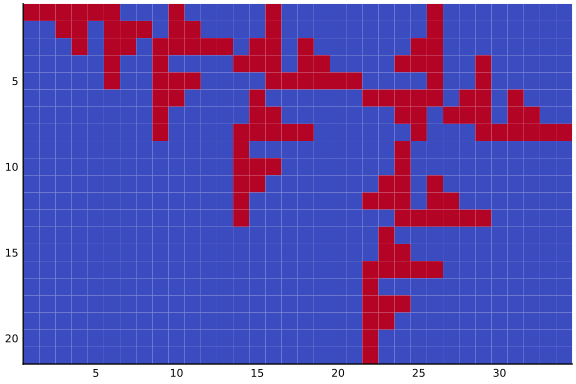
\includegraphics[width=12cm]{media/my-self-rep-frac.png}
\caption{\label{testim}This image is for testing purposes \cite{moskowitzLibraryGuidesWikipedia}}
\end{figure}

\begin{figure}[htbp]
\centering
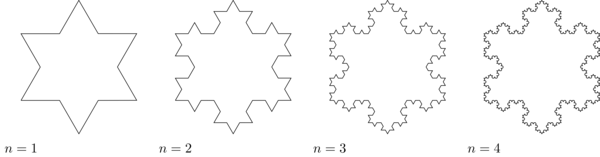
\includegraphics[width=12cm]{media/tikz/Snowflake.png}
\caption{\label{testtikzins}This is a tikz image inserted as a png from imagemagick}
\end{figure}


@@latex: \includestandalone[]{./media/tikz/Snowflake}



\subsection{Heading 2}
\label{heading-2}
\subsubsection{Heading 3}
\label{heading-3}
\begin{minted}[]{sh}
  echo "Hello World"
\end{minted}


\paragraph{Heading 4}
\label{heading-4}
\subparagraph{Heading 5}
\label{heading-5}
\begin{enumerate}
\item Heading 6
\label{heading-6}
Arbitrary Code:

\begin{minted}[]{sh}
  n/bash

  # Print Help
  if [ "$1" == "-h" ]; then
      echo "Usage: `basename $0` <Format> <CSS>"
      style=~/Dropbox/profiles/Emacs/org-css/github-org.css
      exit 0
  fi

  # Make a working File from clipboard
  filename=lkjdskjjalkjkj392jlkj
  xclip -o -selection clipboard >> $filename
  LocalFile=$filename.org

  pandoc -s  -f org -t gfm $filename -o $filename

  echo "
  This was converted from `org` to `md` using `pandoc -t gfm` at time:
  $(date --utc +%FT%H-%M-%S)
  " >> $filename

  cat $filename | xclip -selection clipboard
  rm $filename

  nv & disown
  echo "Conversion from Org Successful, MD is in Clipboard"

  exit 0
\end{minted}
\end{enumerate}
\end{document}
